\documentclass{acm_proc_article-sp}

\usepackage{hyperref}
\usepackage{verbatim}

\begin{document}

\title{Estimating Trust Using Social Networks for Recommendation Systems}


\numberofauthors{1}
\author{
\alignauthor
  Michael Peterson\\
  \affaddr{Carthage College}\\
  \email{mpeterson4@carthage.edu}
}
\date{\today}

\maketitle

\begin{abstract}
  Recommendation systems suggest new items to software developers, but a developer's likelihood to accept a recommendation depends in part on her trust in the person who created the artifact. In this paper, I propose an approach that estimates trust by mining relevant social networks, and an implementation of that approach for GitHub. In a small study, I used the system to estimate trust for all developers in one organization on GitHub.
\end{abstract}

\section{Research Problem \\ and Motivation}
  Among the vast amount of software tools available to developers today, developers use recommendation systems to filter out unimportant data, and retrieve relevant information~\cite{5}. A recommendation system for software engineers (RSSE) is described by Robillard as a system that provides information about a software development task in a given context~\cite{5}.
  For example, a developer may use an RSSE to get recommendations for expert developers, who are knowledgeable about a specific piece of code or about a specific tool, like a static analysis tool.

  Augmenting recommendations with how much a developer is likely to trust another developer may be helpful in improving recommendation adoption~\cite{2}. Using the expert recommendation example, a developer may be more likely to take the recommendation if she trusts the person who is being recommended. Thus, if a system knows how much the developer trusts a set of recommended experts, the system should recommend the one with the highest trust first. Trust-based recommendation systems exist, but they require historical data about a developer's interaction with the system~\cite{3, 4}.

  My main contribution in this paper is designing a system\footnote{System available at \url{http://goo.gl/vM99J5}} to estimate trust, without previous developer interaction, using GitHub.

\section{Background and Related Work}
  \subsection{Defining Trust}
    According to Deutsch \cite{6}, an individual has trust in another individual if he expects him to complete a task. Trust is lost, when the trusted individual does not complete the task. This is the trust one developer has in another, or \textit{developer trust}. From the expert recommendation example, if a developer does not trust a recommended expert to complete their task, they may lose \textit{system trust}, or the amount of trust a developer has in an RSSE. If RSSEs utilized trust from social networks to provide recommendations from a developer's most trusted peers, the developer may have more trust in the system.

  \subsection{Related Work}
    Walter and colleagues~\cite{3} and O'Donovan and Smyth~\cite{4} both describe how social networks can be used as a way to formulate trust for a recommendation system for purchasing items. They describe recommendation systems, for products, that build networks. Users of these networks can gain trust by providing correct reviews of items, and lose trust by providing incorrect reviews. Walter gives a way to estimate correctness by letting users rate user recommendations. O'Donovan measures correctness by predicting the rating of an item, and comparing the prediction with a user's review. Unlike my approach, these approaches require users to have prior interaction with the system.

\section{Approach and Uniqueness}

  I estimated trust by mining information from GitHub. I choose GitHub because it includes a social network for software engineers. The trust between two developers is indicated by a \textit{trust value}. A trust value is an integer, starting at 0, where the higher it is, the higher the trust is. For example, as shown in Table~\ref{tab:trust}, Denis has a trust value of 13 for Linda, and a value of 15 for Brian. There is no threshold to say Denis actually trusts Linda or Brian, rather the amount of trust is used to determine which developer Denis trusts the most. From this, we can conclude that Denis trusts Brian more than he trusts Linda.

  \begin{table}[t]
    \centering
    \begin{tabular}{| c | c | c | c | c |}
      \hline
      Developers  & Denis  & Linda  & Brian  & Emily  \\ \hline
      Denis       & -    & 13     & 15     & 0      \\ \hline
      Linda       & 13     & -    & 15     & 5      \\ \hline
      Brian       & 15     & 11     & -    & 5      \\ \hline
      Emily       & 0      & 1      & 1      & -    \\ \hline
    \end{tabular}
    \caption{An example of developer trust estimated from GitHub.}
    \label{tab:trust}
  \end{table}
  
  My implementation splits trust into four categories, \textit{watching} ($w$), \textit{following} ($f$), \textit{starring} ($s$), and \textit{organization} ($o$). When a developer watches a repository, they get updates to that repository's activity. When Denis follows Linda, he gets updates on her GitHub activity. When a developer stars a repository, they have quick access to it. When a developer is in an organization, they can share projects with other members of the organization. The system estimates a trust value for each category and adds them together for the final trust value. Therefore, the trust value ($t$) formula is as follows:

  \begin{center}
    $ t = w + f + s + o $
  \end{center}

  Each category has a linear equation. Although my system contains placeholders for the constants, they should be machine learned in future work, therefore they will be shown as $ C_n $ in this paper.

  $ w = C_0a + C_1b + C_3d $, where $a$ is the number of repositories Denis is watching that Linda owns, $b$ is the number of repositories Linda is watching that Denis owns, and $d$ is the number of repositories they are mutually following.

  $ f = C_4e + C_5f $, where $e$ is a constant in a set representing a type of follow status, mutual, following, and leader; mutual is when both developers are following each other, following is when Denis follows Linda, leader is when Linda follows Denis. $f$ is a variable representing the number of mutual followers.

  $ s = C_6g + C_7h + C_8i$, where $g$ is the number of repositories Denis has starred that Linda owns, $h$ is the number of repositories Linda has starred that Denis owns, and $i$ is the number of repositories they have both starred.

  $ o = C_9j $, where $j$ is the number of organizations both developers are in.

\section{Results and Contributions}
  \begin{figure}
    \centering
    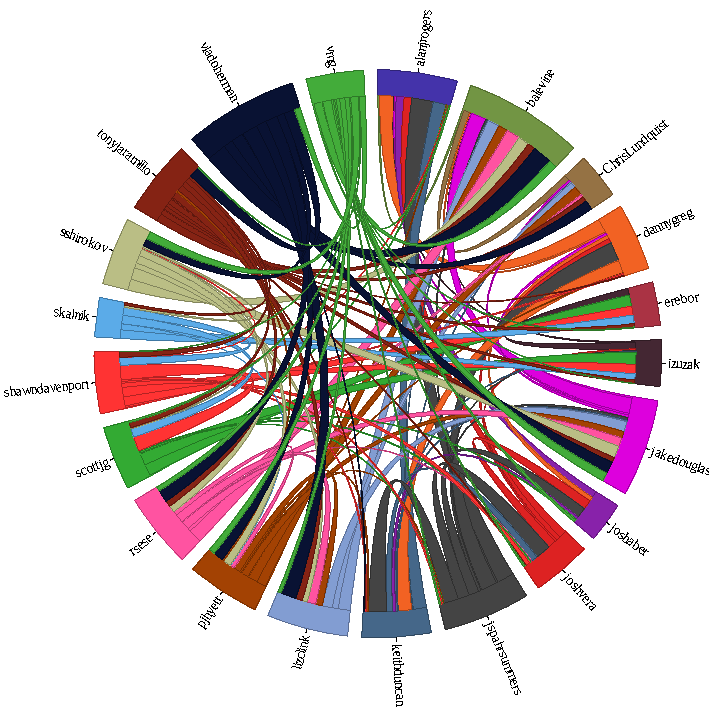
\includegraphics[width=.85\columnwidth, height=.85\columnwidth]{chord-diagram.pdf}
    \caption{Trust diagram of the GitHub organization. }
    \label{fig:trust}
  \end{figure}

  I estimated trust on all 216 developers in the GitHub organization\footnote{\url{https://github.com/github}} on GitHub\footnote{Data available at \url{http://goo.gl/YMnH1f}}. Because the data was too large for a good visualization, I took datasets with different threshold levels for trust values, and removed the trust each developer had for being in the GitHub organization. I then created interactive chord diagrams\footnote{Diagrams available at \url{http://goo.gl/JOicaf}} for each threshold level.

  The color of the paths is the color of the developer who is trusted more within the connection. The thicker the line is at a developer, the more trusted that developer is by their connection.

  As shown in Figure~\ref{fig:trust}, only 21 developers remained with a threshold of 75. Some developers have only a few connections, while others have many. Those with many connections generally have stronger connections as well. Most developers with a stronger trust towards another developer, are also more strongly trusted by that developer. Similarly, a developer with weak trust towards another developer is generally more weakly trusted by that developer.

  \subsection{Limitations}
    A limitation of my research is that the system designed may not extend to every social network. Some social networks do not have concepts such as starring or watching. Because of this, different systems may have to design its own rules for each social network.

  \subsection{Future Work}
    In the future, this system's results could be evaluated, by surveying active developers on GitHub. They could be asked questions such as, how much they worked with a range of their trusted or not trusted GitHub connections, and how much they would trust a recommendation from each of these developers. Then, the data from these surveys could be used to refine the estimation by changing the weights of the constants.

\bibliographystyle{abbrv}
\bibliography{sigproc-sp.bib}

\balancecolumns
\end{document}
